\section{Prefiksne strukture podataka}

\subsection{Prefiksno stablo}

Prefiksno stablo, odnosno \textit{trie} je struktura podataka za \v cuvanje i pretragu kolekcije stringova, i ima oblik $n$-arnog korenskog stabla, odnosno stabla gde svaki \v cvor ima stepen najvi\v se $|\Sigma|$. Kod prefiksnog stabla grane imaju labele koje odgovaraju nekom slovu alfabeta $\Sigma$, dok \v cvorovi \v cuvaju nenegativan ceo broj $c_i$ koji \' cemo zvati \textit{vi\v sestrukost}.

\begin{dfn}
\label{triedef}
Prefiksno stablo za kolekciju stringova $S$ iz alfabeta $\Sigma$ je korensko stablo sa minimalnim brojem \v cvorova, kod kojeg za svaki string $s \in S$ postoji put od korena do \v cvora koji ozna\v cavamo sa $\delta(s)$ tako da labele obi\dj enih grana obrazuju string $s$, a u \v cvoru $\delta(s)$ je vi\v sestrukost jednaka broju pojavljivanja stringa $s$ u kolekciji $S$, i kod kojeg izlazne grane svakog \v cvora imaju me\dj usobno razli\v cite labele.
\end{dfn}

Na osnovu definicije sledi da razli\v citi putevi u stablu koji po\v cinju od istog \v cvora odgovaraju razli\v citim stringovima. Posmatrajmo skup svih prefiksa svih stringova u $S$, neka je to skup $P$. Kako postojanje puta od korena sa labelom $s \in S$ implicira postojanje takvog puta za sve prefikse stringa $s$, va\v zi da \' ce za svaki string $p \in P$ postojati jedinstven \v cvor u stablu. Pokazuje se da je mogu\' ce konstruisati jedinstveno stablo sa ta\v cno $|P|$ \v cvorova koje zadovoljava definiciju \ref{triedef}.

\begin{figure}[H]
    \centering
    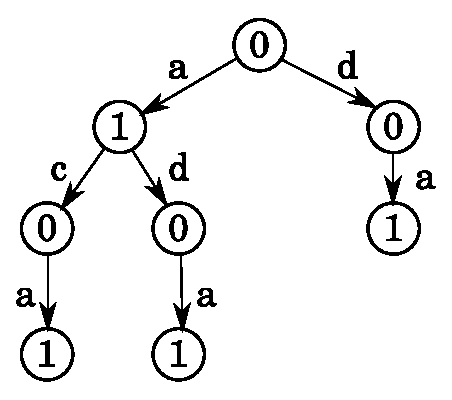
\includegraphics[width=60mm]{../img/trie1.eps}
    \caption*{\textit{Prefiksno stablo za kolekciju $\{aca,ada,a,da\}$.}}
\end{figure}

\subsubsection{Konstrukcija}

Kao \v sto je prethodno opisano, svaki \v cvor u sebi \v cuva vi\v sestrukost, i tako\dj e \' ce \v cuvati izlazne grane. Grane \' ce biti \v cuvane kao kolekcija parova $(k, v)$, gde \' ce $k$ biti slovo, a $v$ pokaziva\v c na \v cvor do kojeg se dolazi tom granom. Ovo je najjednostavnije uraditi pomo\' cu re\v cnika, \v sto nam omogu\'cava brzo umetanje nove grane a tako\dj e i brzu pretragu grane sa odre\dj enim slovom.

\lstinputlisting[language=C++, title={\textit{Struktura \v cvora prefiksnog stabla}}, style=customcpp]{cpp/trie_node.h}

Algoritam za konstrukciju prefiksnog stabla dodaje redom jedan po jedan string iz kolekcije. Pri dodavanju jednog stringa, kre\' cemo se po postoje\' cim granama dokle god je to mogu\' ce, a ukoliko nije kreiramo novi \v cvor. Na kraju se u \v cvoru u kom se zavr\v si kretanje dodaje $1$ na vrednost $c$.

\lstinputlisting[language=C++, title={\textit{Algoritam za dodavanje jednog stringa u prefiksno stablo}}, style=customcpp]{cpp/trie_insert.cpp}

Ukoliko pretpostavimo da operacije na mapi imaju konstantnu slo\v zenost, \v sto je opravdano konstantnom veli\v cinom alfabeta, dolazimo do toga da je vremenska slo\v zenost algoritma linearna po veli\v cini stringa koji se dodaje.

\subsubsection{Primene}

Prefiksno stablo ima veliki broj primena. Svaka od primena mo\v ze zahtevati druga\v ciji izgled strukture jednog \v cvora, ali svima je zajedni\v cko to da \v cvor \v cuva svoje izlazne grane i skelet algoritma za dodavanje stringa je isti kao \v sto je prikazano u kodu gore.

Najosnovnija primena prefiksnog stabla je za implementaciju re\v cnika, odnosno, ono nam omogu\' cava da brzo proverimo da li se neki string javlja u kolekciji ili ne.

\lstinputlisting[language=C++, title={\textit{Algoritam za brojanje pojavljivanja stringa u prefiksnom stablu}}, style=customcpp]{cpp/trie_count.cpp}

Ukoliko pri dodavanju jednog stringa svim usput obi\dj enim \v cvorovima inkrementiramo vi\v sestrukost $c$, prethodni algoritam \' ce vratiti broj stringova u kolekciji koji imaju $s$ kao svoj prefiks, odnosno, mogu\' ce je dodati sve prefikse jednog stringa odjednom, bez pove\' canja vremenske ili memorijske slo\v zenosti.

Mogu\' ce je i prona\' ci leksikografski najmanji string u kolekciji koji je ve\' ci ili jednak zadatom, odnosno, na\' ci \textit{lower bound} za dati string. Za to nam je potrebna pomo\' cna funkcija koja za dati \v cvor nalazi leksikografski najmanji put od tog \v cvora do nekog \v cvora sa pozitivnom vi\v sestruko\v s\' cu. 

\lstinputlisting[language=C++, title={\textit{Algoritam za nala\v zenje najmanjeg stringa po\v cev od zadatog \v cvora}}, style=customcpp]{cpp/trie_smallest.cpp}

Primetimo da $c=0$ implicira da \v cvor ima bar jednu izlaznu granu.

\noindent
\begin{minipage}[l]{\textwidth}
\lstinputlisting[language=C++, title={\textit{Algoritam za nala\v zenje lower bound-a za zadati string}}, style=customcpp]{cpp/trie_lb.cpp}
\end{minipage}

Algoritam je grabljive prirode. Posmatrajmo najdu\v zi zajedni\v cki prefiks stringa $s$ za koji tra\v zimo \textit{lower bound} i nekog stringa iz kolekcije. Ukoliko je taj prefiks jednak celom stringu $s$, potrebno je da na\dj emo najmanji string $q$ dosti\v zan iz \v cvora $\delta(s)$, i da vratimo $sq$. U suprotnom, ako je du\v zina tog zajedni\v ckog prefiksa $i$, biramo najve\' cu poziciju $j \leq i$ takvu da u \v cvoru $\delta(s_{[0, j)})$ postoji izlazna grana \v cija je labela slovo strogo ve\' ce od $s_j$, zatim vra\' camo string $s_{[0,j)}yq$, gde je $y$ to slovo a $q$ najmanji string dosti\v zan iz \v cvora $\delta(s_{[0,j)}y)$. Ukoliko takav indeks ne postoji, ne postoji ni leksikografski ve\' ci ili jednak string, a algoritam vra\' ca prazan string.

\textit{Primer.} Neka je kolekcija stringova $\{aba, ada, adc, bu\}$, a tra\v zimo \textit{lower bound} za string $abo$. Prvo tra\v zimo najdu\v zi prefiks stringa $abo$ koji se nalazi u stablu, to je string $ab$.

\begin{figure}[H]
    \centering
    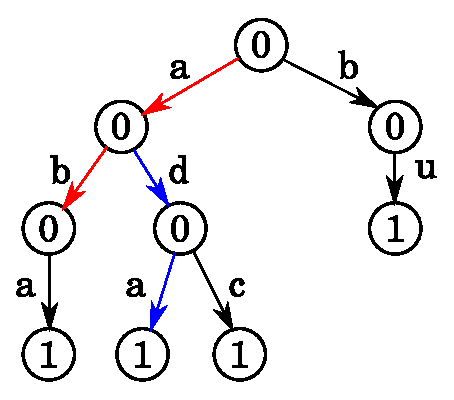
\includegraphics[width=60mm]{../img/trielb1.eps}
\end{figure}

Kako nismo do\v sli do kraja celog stringa, vra\' camo se unazad kroz stablo, sve dok ne na\dj emo \v cvor koji ima izlaznu granu sa labelom strogo ve\' com od odgovaraju\' ceg slova u stringu $abo$. Nalazimo takvu granu u \v cvoru $\delta(a)$, a zatim se grabljivim postupkom spu\v stamo sve do nekog \v cvora sa pozitivnom vi\v sestruko\v s\' cu, \v sto je u ovom slu\v caju \v cvor $\delta(ada)$, pa je rezultat upravo string $ada$.

Ukupna memorijska i vremenska slo\v zenost celog algoritma je $O(n+m)$. gde je $n = |s|$, a $m$ je du\v zina rezultuju\' ceg stringa.

\subsection{Aho-Corasick algoritam}

Aho-Corasick algoritam omogu\' cava pretragu vi\v se stringova odjednom, odnosno, za dati skup nepraznih stringova $P$ i string $s$, on pronalazi sva pojavljivanja svih stringova iz $P$ u $s$. Kako je ukupan broj pojavljivanja svih stringova u najgorem slu\v caju srazmeran $|s|\cdot|P|$, tako je i ovo donja granica na slo\v zenost bilo kog algoritma koji pronalazi sva pojavljivanja.

Aho-Corasick algoritam generalizuje KMP algoritam. Osnova za ovaj algoritam je upravo prefiksno stablo i prvi korak jeste njegova konstrukcija, uz malu modifikaciju, koja se odnosi na postojanje dodatnih polja, koje se zovu \textit{sufiks veza} i \textit{re\v cni\v cka veza}. Tako\dj e, umesto vi\v sestrukosti, za \v cvor $\delta(p)$ pamtimo $id$, odnosno redni broj stringa $p \in P$, ukoliko se ne radi o stringu iz $P$ ve\' c o nekom prefiksu, upisujemo $id = -1$. 

\noindent
\begin{minipage}[l]{\textwidth}
\lstinputlisting[language=C++, title={\textit{Struktura \v cvora kod Aho-Corasick algoritma}}, style=customcpp]{cpp/aho_node.h}
\end{minipage}

\noindent
\begin{minipage}[l]{\textwidth}
\lstinputlisting[language=C++, title={\textit{Dodavanje stringa u prefiksno stablo kod Aho-Corasick algoritma}}, style=customcpp]{cpp/aho_insert.cpp}
\end{minipage}

\begin{dfn}
Za prefiksno stablo izgra\dj eno od skupa stringova $P$, sufiks veza \v cvora $\delta(s)$ pokazuje na \v cvor $\delta(q)$ takav da je $q$ najdu\v zi string koji je prefiks nekog stringa u $P$, a koji je ujedno pravi sufiks stringa $s$. Za koren se sufiks veza ne defini\v se.
\end{dfn}

Primetimo da za jednoelementni skup $P$ ove sufiks veze ta\v cno odgovaraju nizu neuspeha kod KMP algoritma. Sufiks veza nekog \v cvora uvek pokazuje na \v cvor strogo manje dubine. Zbog ovoga, \v cvorove je neophodno obraditi u redosledu sortiranom po dubini, za \v sta se koristi pretraga u \v sirinu. Prirodno, algoritam za nala\v zenje sufiks veza podse\' ca na prvu fazu KMP algoritma. Za svaki \v cvor $p$, kre\' cemo od sufiks veze njegovog roditelja $t$, i tra\v zimo \v cvor $l$ koji ima izlaznu granu sa istom labelom kao grana koja spaja $t,p$. Pretragu vr\v simo pra\' cenjem sufiks veza. Ukoliko na\dj emo takav \v cvor, sufiks veza \v cvora $p$ \' ce pokazivati na odgovaraju\' ce dete \v cvora $l$, u suprotnom, sufiks veza pokazuje na koren.

\noindent
\begin{minipage}[l]{\textwidth}
\lstinputlisting[language=C++, title={\textit{Nala\v zenje sufiks veza kod Aho-Corasick algoritma}}, style=customcpp]{cpp/aho_find_links.cpp}
\end{minipage}

Funkcija vra\' ca niz svih \v cvorova stabla, sortiran po dubini. Ovaj niz \' ce biti koristan u kasnijoj obradi. Neka je $L$ ukupna du\v zina svih stringova u $P$. Vremenska slo\v zenost nala\v zenja svih sufiks veza je $O(L)$\cite{ahorad}. Dokaz je sli\v can dokazu slo\v zenosti kod KMP algoritma.

\begin{figure}[H]
    \centering
    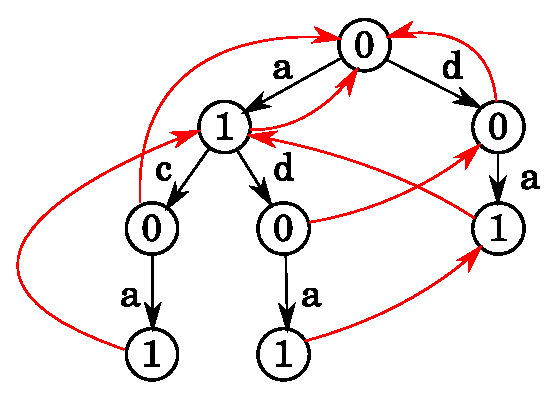
\includegraphics[width=75mm]{../img/aho1.eps}
    \caption*{\textit{Sufiks veze za prefiksno stablo za kolekciju $\{aca,ada,a,da\}$.}}
\end{figure}

Prefiksno stablo podse\' ca na deterministi\v cki kona\v cni automat, jer ima jedan polazni \v cvor i svaki \v cvor ima izlazne grane ozna\v cene simbolima iz alfabeta $\Sigma$. Me\dj utim, neki \v cvorovi, npr. listovi stabla nemaju izlazne grane za svaki simbol $x \in \Sigma$. Pomo\' cu izra\v cunatih sufiks veza mo\v zemo dopuniti stablo do pravog kona\v cnog automata. Neka je $u$ proizvoljan \v cvor stabla, a $x \in \Sigma$ proizvoljan simbol. Po\v cev od \v cvora $u$, uklju\v cuju\' ci i $u$, kre\' cemo se po sufiks vezama i tra\v zimo prvi \v cvor koji ima izlaznu granu sa labelom $x$. Ukoliko takav \v cvor ne postoji, grana automata sa labelom $x$ iz $u$ ide ka korenu stabla. U suprotnom, neka je to \v cvor $v$. Tada ta grana ide ka \v cvoru na koji pokazuje grana sa labelom $x$ iz \v cvora $v$.

Smisao ovakve definicije automata je slede\' ci. Ukoliko se kroz automat propusti string $s$, ako se automat nalazi u stanju $\delta(p)$, tada je $p$ najdu\v zi prefiks nekog stringa iz $P$ koji je ujedno sufiks stringa $s$. Tada je ovakva definicija automata valjana, odnosno, ovako definisan automat zaista raspoznaje sve razli\v cite prefikse stringova iz $P$. Zbog ovakve definicije, nije nu\v zno eksplicitno pamtiti sve prelaze automata -- dovoljno je pri svakom prelazu potra\v ziti pomo\' cu sufiks veza odgovaraju\' ci \v cvor. Sli\v cno kao kod KMP-a, ukoliko se kroz ovaj automat propusti string $s$, ukupna vremenska slo\v zenost za kretanje kroz automat \' ce biti $O(|s|)$. \cite{ahorad}

Po\v sto svaka sufiks veza ide od \v cvora ve\' ce ka \v cvoru manje dubine, graf koji obrazuju ove veze je acikli\v can, a po\v sto svaki \v cvor osim ta\v cno jednog ima izlaznu granu, radi se o obrnutom korenskom stablu. Nadalje \' cemo ovo stablo zvati \textit{stablo sufiks veza}. I originalni Aho-Corasick algoritam i njegove modifikacije se oslanjaju na preprocesiranje ovog stabla.

Originalni Aho-Corasick algoritam nalazi, za skup stringova $P$ i svaki prefiks $s_{[0,i)}$ stringa $s$ sve stringove $p \in P$ koji su sufiksi stringa $s_{[0,i)}$, u vremenskoj slo\v zenosti $O(L+|s|+k)$, gde je $k$ broj poklapanja. Posmatrajmo \v sta se de\v sava nakon ta\v cno $i$ prelaza, odnosno, kada smo stigli do prefiksa $s_{[0,i)}$. Neka se automat nalazi u stanju $\delta(q)$. Posmatrajmo put od \v cvora $q$ do korena kroz stablo sufiks veza. Svaki \v cvor na ovom putu koji ima pozitivnu vi\v sestrukost odgovara pojavljivanju nekog stringa $p \in P$ kao sufiks stringa $s_{[0,i)}$. Dakle, na\v s cilj treba da bude da efikasno otkrijemo sve ove \v cvorove, po\v zeljno u linearnoj slo\v zenosti po njihovom broju. Zato uvodimo novi tip veze -- re\v cni\v cku vezu.

\begin{dfn}
Re\v cni\v cka veza za \v cvor $u$ stabla sufiks veza je prvi \v cvor dosti\v zan iz $u$ kod kojeg je vi\v sestrukost pozitivna. Ukoliko takav \v cvor ne postoji, re\v cni\v cka veza se ne defini\v se.
\end{dfn}

Re\v cni\v cke veze nam omogu\' cavaju da presko\v cimo sve usputne \v cvorove koji ne odgovaraju celim stringovima iz $P$, odnosno, da direktno obi\dj emo sve \v cvorove sa pozitivnom vi\v sestruko\v s\' cu. Ove veze se jednostavno konstrui\v su ukoliko je ve\' c izra\v cunat niz \v cvorova sortiran po dubini.

\noindent
\begin{minipage}[l]{\textwidth}
\lstinputlisting[language=C++, title={\textit{Nala\v zenje re\v cni\v ckih veza kod Aho-Corasick algoritma}}, style=customcpp]{cpp/aho_find_dict.cpp}
\end{minipage}

Niz $q$ je prethodno izra\v cunati niz \v cvorova, jasno je da je $q_0$ koren i da je on jedini \v cvor koji nema sufiks vezu. Za sve ostale \v cvorove va\v zi da, ako oni imaju pozitivnu vi\v sestrukost, onda re\v cni\v cka veza pokazuje upravo na njih same, a ina\v ce \' ce pokazivati na isti \v cvor na koji pokazuje njihova sufiks veza.

Kona\v cno, opi\v simo rad celog algoritma. Prvo, konstrui\v semo prefiksno stablo ubacivanjem svih stringova iz $P$. Zatim nalazimo sufiks veze i re\v cni\v cke veze. Zatim, obra\dj ujemo string $s$, u svakom trenutku pamtimo pokaziva\v c na trenutnu poziciju u automatu. Nakon svakog dodatog slova, pomo\' cu re\v cni\v ckih veza obi\dj emo sva sufiksna poklapanja sa stringovima iz $P$.

\noindent
\begin{minipage}[l]{\textwidth}
\lstinputlisting[language=C++, title={\textit{Glavna funkcija Aho-Corasick algoritma}}, style=customcpp]{cpp/aho_main.cpp}
\end{minipage}

Na osnovu svega do sad opisanog, slo\v zenost algoritma je linearna po zbiru veli\v cina ulaza i izlaza. Jedan od nedostataka ovakvog pristupa je \v sto izlaz mo\v ze biti dosta veliki, na primer, ako je $P = \{a, a^2, \ldots, a^k\}$ a $s = a^n$, ukupna veli\v cina ulaza je $\Theta(k^2+n)$ dok je veli\v cina izlaza $\Theta(kn)$, \v sto je za, na primer $k = \Theta(\sqrt{n})$ superlinearna funkcija du\v zine ulaza. Ukoliko je potrebno eksplicitno enumerisati sva pojavljivanja prethodno opisani algoritam je optimalan. U suprotnom, mogu\' ce varijacije su da treba da se prijavi broj pojavljivanja ili prvo pojavljivanje svakog stringa $p \in P$ u $s$. Ovo je mogu\' ce posti\' ci u linearnom vremenu po veli\v cini ulaza modifikacijom glavnog algoritma. Naime, za svaki \v cvor prefiksnog stabla zapamtimo sve trenutke $i$ kada smo, nakon obrade prefiksa $s_{[0, i)}$ zavr\v sili ba\v s u tom \v cvoru. Broj pojavljivanja nekog stringa $p \in P$ je onda ukupan broj trenutaka kada smo bili u podstablu stabla sufiks veza sa korenom u \v cvoru $\delta(p)$, dok je prvo pojavljivanje jednako minimumu svih trenutaka pojavljivanja u tom podstablu. Obe ove vrednosti se mogu efikasno izra\v cunati postprocesiranjem stabla nakon obilaska celog stringa $s$, primenom dinami\v ckog programiranja.
